\chapter{Solution of nonlinear systems}
\label{cha:solution_of_nonlinear_systems}
\minitoc

\section*{Introduction}

This chapter concerns the numerical solution of nonlinear equations of the general form
\begin{equation}
    \label{eq:nonlinear_equation}
    \vect f(\vect x) = 0, \qquad \vect f\colon \real^n \to \real^n.
\end{equation}
A solution to this equation is called a \emph{zero} of the function $f$.
Except in particular cases (for example linear systems),
there does not exist a numerical method for solving~\eqref{eq:nonlinear_equation} in a finite number of operations,
so iterative methods are required.

In contrast with the previous chapter,
it may not be the case that~\eqref{eq:nonlinear_equation} admits one and only one solution.
For example, the equation $1 + x^2 = 0$ does not have a (real) solution,
and the equation $\cos(x) = 0$ has infinitely many.
Therefore, convergence results usually contain assumptions on the function~$f$ that guarantee the existence and uniqueness of a solution in~$\real^n$ or a subset of~$\real^n$.

For an iterative method generating approximations $(\vect x_k)_{k \geq 0}$ of a root $\vect x_*$,
we define the error as $\vect e_k = \vect x_k - \vect x_*$.
If the sequence $(\vect x_k)_{k \geq 0}$ converges to $\vect x_*$ in the limit as $k \to \infty$
and if
\begin{equation}
    \label{eq:rate_of_convergence}
    \lim_{k \to \infty} \frac{\norm{\vect e_{k+1}}}{\norm{\vect e_k}^q} = r,
\end{equation}
then we say that $(\vect x_k)_{k \geq 0}$ converges with \emph{order of convergence} $q$ and
\emph{rate of convergence} $r$.
In addition, we say that the convergence is linear $q = 1$,
and quadratic if $q = 2$.
The convergence is said to be superlinear if
\begin{equation}
    \label{eq:superlinear}
    \lim_{k \to \infty} \frac{\norm{\vect e_{k+1}}}{\norm{\vect e_k}} = 0.
\end{equation}
In particular,
the convergence is superlinear if the order of convergence is $q > 1$.

\begin{remark}
    The notion of order of convergence may be defined also when
    the limit in~\eqref{eq:rate_of_convergence} does not exist.
    A more general definition for the order of convergence of a sequence~$(\vect x_k)_{k\geq0}$ converging to $\vect x_*$ is the following:
    \[
        q(\vect x_0) = \inf \left\{ p \in [1, \infty) : \limsup_{k \to \infty} \frac{\norm{\vect e_{k+1}}}{\norm{\vect e_k}^p} = \infty \right\},
    \]
    or $q(\vect x_0) = \infty$ if the numerator and denominator of the fraction are zero for sufficiently large~$k$.
    It is possible to define similarly the order of convergence of an iterative method
    for an initial guess in a neighborhood $V$ of $\vect x_*$:
    \[
        q = \inf \left\{ p \in [1, \infty) : \sup_{\vect x_0 \in V} \left( \limsup_{k \to \infty} \frac{\norm{\vect e_{k+1}}}{\norm{\vect e_k}^p} \right) = \infty \right\},
    \]
    where the fraction should be interpreted as 0 if the numerator and denominator are zero.
    A more detailed discussion of this subject is beyond the scope of this course.
\end{remark}

The rest of chapter is organized as follows:
\begin{itemize}
    \item
        In \cref{sec:bisection_method},
        by way of introduction to the subject of numerical methods for nonlinear equations,
        we present and analyze the bisection method.

    \item
        In \cref{sec:fixed_point_methods},
        we present a general method based on a fixed point iteration for solving~\eqref{eq:nonlinear_equation}.
        The convergence of this method is analyzed in~\cref{sec:convergence_fixed_point_methods}.

    \item
        In \cref{sec:examples_of_fixed_point_methods},
        two concrete examples of fixed point methods are studied:
        the chord method and the Newton--Raphson method.
\end{itemize}

\section{The bisection method}
\label{sec:bisection_method}
As an introduction to numerical methods for solving nonlinear equations,
we present the bisection method.
This method applies only in the case of a real-valued function $f\colon \real \to \real$,
and relies on the knowledge of two points $a < b$ such that $f(a)$ and $f(b)$ have different signs.
By the intermediate value theorem,
there necessarily exists $x_* \in (a, b)$ such that $f(x_*) = 0$.
The idea of the bisection method it to successively divide the interval in two equal parts,
and to retain, based on the sign of $f$ at the midpoint $x_{1/2}$,
the one that necessarily contains a root.
If $f(x_{1/2}) f(a) \geq 0$, then $f(x_{1/2}) f(b) \leq 0$ and so there necessarily exists a root of $f$ in the interval $[x_{1/2}, b)$ by the intermediate value theorem.
In contrast, if $f(x_{1/2}) f(a) < 0$, then there necessarily is a root in the interval $(a, x_{1/2})$.
The algorithm is presented in \cref{algo:bisection}.
\begin{algorithm}
\caption{Bisection method}%
\label{algo:bisection}%
\begin{algorithmic}
\State Assume that $f(a) f(b) < 0$ with $a < b$.
\State Pick $\varepsilon > 0$.
\State $x \gets a/2 + b/2$
\While{$|b - a| \geq \varepsilon$}
    \If{$f(x) f(a) \geq 0$}
        \State $a \gets x$
    \Else
        \State $b \gets x$
    \EndIf
    \State $x \gets a/2 + b/2$
\EndWhile
\end{algorithmic}
\end{algorithm}

The following result establishes the convergence of the method.
\begin{proposition}
    \label{proposition:convergence_bisection}
    Assume that $f\colon \real \to \real$ is a continuous function and $f(a) f(b) < 0$.
    Let~$[a_j, b_j]$ denote the interval obtained after $j$ iterations of the bisection method,
    and let $x_j = (a_j + b_j)/2$ denote the midpoint of the interval,
    Then there exists a root~$x_*$ of $f$ such that
    \begin{equation}
        \label{eq:error_bisection}
        \abs{x_j - x_*} \leq (b_0 - a_0) 2^{-(j+1)}.
    \end{equation}
\end{proposition}
\begin{proof}
    By construction, $f(a_j) f(b_j) \leq 0$ and $f(b) \neq 0$.
    Therefore, by the intermediate value theorem,
    there exists a root of $f$ in the interval $[a_j, b_j)$,
    implying that
    \[
        \abs{x_j - x_*} \leq \frac{b_j - a_j}{2}.
    \]
    Since $b_j - a_j = 2^{-j} (b_0 - a_0)$,
    the statement follows.
\end{proof}
Although the limit in~\eqref{eq:rate_of_convergence} may not be well-defined (for example, $x_1$ may be a root of~$f$),
the error $x_j - x_*$ is bounded in absolute value by the sequence $(\widetilde e_j)_{j \geq 0}$,
where $\widetilde e_j = (b_0 - a_0) 2^{-(j+1)}$ by \cref{proposition:convergence_bisection}.
Since the latter sequence exhibits linear convergence to 0,
the convergence of the bisection method is said to be linear,
by a slight abuse of terminology.

% \section{Convergence speed}
% The definition~\eqref{eq:rate_of_convergence} for the rate of convergence is not completely satisfactory,
% because the limit on the left-hand side may not have exist.
% It is therefore preferable to replace the limit in the definition by a \emph{limit superior}.

\section{Fixed point methods}
\label{sec:fixed_point_methods}

Let $\vect x_*$ denote a zero of the function $\vect f$.
The idea of iterative methods for~\eqref{eq:nonlinear_equation} is to construct,
starting from an initial guess $\vect x_0$,
a sequence $(\vect x_k)_{k=0, 1, \dotsc}$ approaching~$\vect x_*$.
A number of iterative methods for solving ~\eqref{eq:nonlinear_equation} are based on an iteration of the form
\begin{equation}
    \label{eq:fixed_point}
    \vect x_{k+1} = \vect F(\vect x_{k}),
\end{equation}
for an appropriate continuous function $F$.
Assume that $\vect x_k$ converges to some point $\vect x_* \in \real^n$ in the limit as $k \to \infty$.
Then, taking the limit $k \to \infty$ in~\eqref{eq:fixed_point},
we find that $\vect x_*$ satisfies
\[
    \vect F(\vect x_*) = \vect x_*.
\]
Such a point~$\vect x_*$ is called a \emph{fixed point} of the function $\vect F$.
Several definitions of the function~$\vect F$ can be employed in order to ensure that
a fixed point of $\vect F$ coincides with a zero of $\vect f$.
One may, for example, define $\vect F(\vect x) = \vect x - \alpha^{-1} \vect f(\vect x)$,
for some nonzero scalar coefficient $\alpha$.
Then~$\vect F(\vect x_*) = \vect x_*$ if and only if $\vect f(\vect x_*) = 0$.
Later in this chapter,
in \cref{sec:examples_of_fixed_point_methods},
we study two instances of numerical methods which can be recast in the form~\eqref{eq:fixed_point}.
Before this,
we study the convergence of the iteration~\eqref{eq:fixed_point} for a general function~$\vect F$.

\section{Convergence of fixed point methods}
\label{sec:convergence_fixed_point_methods}
Equation~\eqref{eq:fixed_point} may be viewed as a \emph{discrete-time} dynamical system.
In order to study the behavior of the system as $k \to \infty$,
it is important to understand the concept of stability of a fixed point.
The concept of stability appears also in the field of ordinary differential equations,
which are \emph{continuous-time} dynamical systems.
Before we define this concept,
we introduce the following notation
for the open ball of radius $\delta$ around $\vect x \in \real^n$:
\[
    B_{\delta} (\vect x) := \bigl\{ \vect y \in \real^n : \norm{\vect y - \vect x} < \delta \bigr\}.
\]
\vspace{-.7cm}
\begin{definition}
    [Stability of fixed points]
    Let $(\vect x_k)_{k\geq0}$ denote iterates obtained from~\eqref{eq:fixed_point} when starting from an initial vector~$\vect x_0$.
    Then we say that a fixed point $\vect x_*$ is
    \begin{itemize}
        \item
            an \emph{attractor} if there exists a neighborhood $\mathcal V$ of $s$ such that
            \begin{equation}
                \label{eq:nonlinear_attractor}
                \forall \vect x_0 \in \mathcal V, \qquad
                \vect x_k \xrightarrow[k \to \infty]{} \vect x_*.
            \end{equation}
            The largest neighborhood for which this is true,
            i.e. the set of values of $\vect x_0$ such that~\eqref{eq:nonlinear_attractor} holds true,
            is called the basin of attraction of $\vect x_*$.

        \item
            stable (in the sense of Lyapunov) if for all $\varepsilon > 0$,
            there exists $\delta > 0$ such that
            \[
                \forall \vect x_0 \in B_{\delta}(\vect x_*), \qquad
                \forall k \in \nat, \qquad
                \norm{\vect x_k - \vect x_*} < \varepsilon.
            \]

        \item
            asymptotically stable if it is stable and an attractor.

        \item
            exponentially stable if there exists $C > 0$, $\alpha \in (0, 1)$, and $\delta > 0$ such that
            \[
                \forall \vect x_0 \in B_{\delta}(\vect x_*),
                \quad \forall k \in \nat, \qquad
                \norm{\vect x_k - \vect x_*} \leq C \alpha^k \norm{\vect x_0 - \vect x_*}.
            \]

        \item
            globally exponentially stable if there exists $C > 0$ and $\alpha \in (0, 1)$ such that
            \[
                \forall \vect x_0 \in \real^n,
                \quad \forall k \in \nat, \qquad
                \norm{\vect x_k - \vect x_*} \leq C \alpha^k \norm{\vect x_0 - \vect x_*}.
            \]
        \item
            unstable if it is not stable.
    \end{itemize}
\end{definition}
Clearly, global exponential stability implies exponential stability,
which itself implies asymptotic stability and stability.
If $\vect x_*$ is globally exponentially stable,
then $\vect x_*$ is the unique fixed point of~$\vect F$;
showing this is the aim of~\cref{exercise:global_exponential_stability}.
If $\vect x_*$ is an attractor,
then the dynamical system~\eqref{eq:fixed_point} is said to be locally convergent to~$\vect x_*$.
The larger the basin of attraction of $\vect x_*$,
the less careful we need to be when picking the initial guess~$\vect x_0$.
Global exponential stability of a fixed point can sometimes be shown
provided that $\vect F$ satisfies a strong hypothesis.

\begin{definition}
    [Lipschitz continuity]
    A function $\vect F\colon \real^n \to \real^n$ is said to be \emph{Lipschitz} continuous
    with constant $L$ if
    \[
        \forall (\vect x, \vect y) \in \real^n \times \real^n, \qquad
        \norm[big]{\vect F(\vect y) - \vect F(\vect x)} \leq L \norm{\vect y - \vect x}.
    \]
\end{definition}
A function $\vect F\colon \real^n \to \real^n$ that is Lipschitz continuous with a constant $L < 1$ is called a \emph{contraction}.
For such a function, it is possible to prove that~\eqref{eq:fixed_point} has a unique globally exponentially stable fixed point.
\begin{theorem}
    \label{theorem:exponenital_convergence_fixed_point}
    Assume that $\vect F$ is a contraction.
    Then there exists a unique fixed point of~\eqref{eq:fixed_point},
    and it holds that
    \begin{equation}
        \label{eq:global_exp}
        \forall \vect x_0 \in \real^n,
        \quad \forall k \in \nat, \qquad
        \norm{\vect x_k - \vect x_*} \leq L^k \norm{\vect x_0 - \vect x_*}.
    \end{equation}
\end{theorem}
\begin{proof}
    We prove first existence of the fixed point,
    then uniqueness, and finally~\eqref{eq:global_exp}.

    \noindent\textbf{Existence.}
    It holds that
    \[
        \norm[big]{\vect x_{k+2} - \vect x_{k+1}}
        = \norm[big]{\vect F(\vect x_{k+1}) - \vect F(\vect x_k)}
        \leq L\norm{\vect x_{k+1} - \vect x_k}
        \leq \dots \leq L^{k+1} \norm{\vect x_{1} - \vect x_0}.
    \]
    Therefore, for any $n \geq m$,
    we have by the triangle inequality
    \begin{align*}
        \norm{\vect x_{n} - \vect x_{m}}
        &\leq \norm{\vect x_{n} - \vect x_{n-1}} + \dotsb + \norm{\vect x_{m+1} - \vect x_{m}} \\
        &\leq (L^{n-1} + \dotsb + L^{m}) \norm{\vect x_{1} - \vect x_0}
        \leq L^{m} (1 + L + \dotsb) \norm{\vect x_{1} - \vect x_0}
        = \frac{L^{m}}{1-L} \norm{\vect x_{1} - \vect x_0}.
    \end{align*}
    It follows that the sequence $(\vect x_k)_{k\geq0}$ is Cauchy in $\real^n$,
    implying by completeness that $\vect x_k \to \vect x_*$ in the limit as $k \to \infty$,
    for some limit $\vect x_* \in \real^n$.
    Being a contraction, the function $\vect F$ is continuous,
    and so taking the limit~$k \to \infty$ in~\eqref{eq:fixed_point}, we obtain that
    \[
        \vect x_* = \lim_{k \to \infty} \vect x_{k+1}
        = \lim_{k \to \infty} \vect F(\vect x_k)
        = \vect F \left( \lim_{k \to \infty} \vect x_k \right)
        = \vect F(\vect x_*).
    \]
    In other words, $\vect x_*$ is a fixed point of~$\vect F$.

    \vspace{.2cm}
    \noindent\textbf{Uniqueness.}
    Assume that $\vect y_*$ is another fixed point.
    Then,
    \begin{equation*}
        \norm[big]{\vect y_* - \vect x_{*}}
        = \norm[big]{\vect F(\vect y_*) - \vect F(\vect x_{*})}
        \leq L \norm{\vect y_* - \vect x_*},
    \end{equation*}
    which implies that $\vect y_* = \vect x_*$ since $L < 1$.

    \vspace{.2cm}
    \noindent\textbf{Global exponential convergence.}
    Since $\vect F$ is a contraction,
    it holds that
    \begin{equation}
        \label{eq:contraction}
        \norm[big]{\vect x_{k} - \vect x_{*}}
        = \norm[big]{\vect F(\vect x_{k-1}) - \vect F(\vect x_*)}
        \leq L\norm{\vect x_{k-1} - \vect x_*}
        \leq \dots \leq L^{k} \norm{\vect x_{0} - \vect x_*},
    \end{equation}
    which proves~\eqref{eq:global_exp}.
\end{proof}

It is possible to prove a weaker, local result under a less restrictive assumptions on the function~$\vect F$.
\begin{theorem}
    \label{theorem:local_convergence}
    Assume that $\vect x_*$ is a fixed point of~\eqref{eq:fixed_point} and that $\vect F\colon \real^n \to \real^n$ satisfies the local Lipschitz condition
    \begin{equation}
        \label{eq:local_lipschitz}
        \forall \vect x \in B_{\delta}(\vect x_*), \qquad
        \norm[big]{\vect F(\vect x) - \vect F(\vect x_*)} \leq L \norm{\vect x - \vect x_*},
    \end{equation}
    with $0 \leq L < 1$ and $\delta > 0$.
    Then~$\vect x_*$ is the unique fixed point of~$\vect F$ in $B_{\delta}(\vect x_*)$ and,
    for all~$\vect x_0 \in B_{\delta}(\vect x_*)$, it holds that
    \begin{itemize}
        \item All the iterates $(\vect x_k)_{k \in \nat}$ belong to $B_{\delta}(\vect x_*)$.
        \item The sequence $(\vect x_k)_{k \in \nat}$ converges exponentially to $\vect x_*$.
    \end{itemize}
\end{theorem}
\begin{proof}
    See~\cref{exercise:prove_local_convergence}.
\end{proof}
It is possible to guarantee that condition~\eqref{eq:local_lipschitz} holds provided that
we have sufficiently good control of the derivatives of the function~$\vect F$.
The function $\vect F$ is said to be differentiable at $\vect x$ (in the sense of Fréchet) if
there exists a linear operator $\D \vect F_{\vect x} \colon \real^n \to \real^n$ such that
\begin{equation}
    \label{eq:limit_differentiability}
    \lim_{\vect h \to 0} \frac{\norm{\vect F(\vect x + \vect h) - \vect F(\vect x) - \D \vect F_{\vect x}(\vect h)}}{\norm{\vect h}}
    = 0.
\end{equation}
If $\vect F$ is differentiable,
then all its first partial derivatives~$\partial_j F_i$ exist and,
in addition, it holds that $\D \vect F_{\vect x}(\vect h) = \mat J_F(\vect x) \vect h$
where $\mat J_F(\vect x)$ is the Jacobian matrix of~$\vect F$ at $\vect x$:
\[
    \mat J_F(\vect x) =
    \begin{pmatrix}
        \partial_{1} F_1(\vect x) & \hdots & \partial_n F_1(\vect x) \\
        \vdots & \ddots & \vdots \\
        \partial_{1} F_n(\vect x) & \hdots & \partial_n F_n(\vect x)
    \end{pmatrix}.
\]

\begin{proposition}
    \label{proposition:local_convergence_fixed_point}
    Let $\vect x_*$ be a fixed point of~\eqref{eq:fixed_point},
    and assume that there exists $\delta$ and a subordinate matrix norm such that
    $\vect F$ is differentiable everywhere in $B_{\delta}(\vect x_*)$ and
    \[
        \forall \vect x \in B_{\delta}(\vect x_*), \qquad
        \norm{\mat J_F(\vect x)} \leq L < 1.
    \]
    Then condition~\eqref{eq:local_lipschitz} is satisfied in the associated vector norm,
    and so the fixed point $\vect x_*$ is locally exponentially stable.
\end{proposition}
\begin{proof}
    Let $\vect x \in B_{\delta}(\vect x_*)$.
    By the fundamental theorem of calculus and the chain rule,
    we have
    \begin{align*}
        \vect F(\vect x) - \vect F(\vect x_*)
        &= \int_{0}^{1} \frac{\d}{\d t} \Bigl( \vect F\bigl(\vect x_* + t(\vect x - \vect x_*) \bigr) \Bigr) \d t
        = \int_{0}^{1} \mat J_F\bigl(\vect x_* + t(\vect x - \vect x_*)\bigr) \left(\vect x - \vect x_* \right) \d t.
    \end{align*}
    Therefore,
    it holds that
    \begin{align*}
        \norm{\vect F(\vect x) - \vect F(\vect x_*)}
        \leq \int_{0}^{1} \norm*{\mat J_F\bigl(\vect x + t(\vect x - \vect x_*)\bigr)}  \, \d t \, \norm{\vect x - \vect x_*}
        \leq \int_{0}^{1} L \, \d t \, \norm{\vect x - \vect x_*} = L \norm{\vect x - \vect x_*},
    \end{align*}
    which is the statement.
\end{proof}
\begin{remark}
    As Hannah observed during the lecture,
    in dimension~$n = 1$, \cref{proposition:local_convergence_fixed_point} can be proved by using the mean value theorem:
    since $F$ is differentiable in~$(x_* -\delta, x_* + \delta)$,
    there exists for all $x$ in this interval a $\xi = \xi(x)$ also in this interval such that
    \[
        F(x) - F(x_*) = F'(\xi) (x - x_*).
    \]
    It then follows immediately that
    \[
        \bigl\lvert F(x) - F(x_*) \bigr\rvert
        = \left\lvert F'(\xi) (x - x_*) \right\rvert
        \leq L \lvert x - x_* \rvert.
    \]
    This proof does not carry over to the multi-dimensional setting, however.
\end{remark}

In fact, it is possible to prove that a fixed point~$\vect x_*$ is exponentially locally stable under an even weaker condition,
involving only the derivative of $\vect F$ at $\vect x_*$.
\begin{proposition}
    \label{proposition:local_convergence}
    Let $\vect x_*$ be a fixed point of~\eqref{eq:fixed_point} and that $f$ is differentiable at $\vect x_*$ with
    \[
        \norm{\mat J_F(\vect x_*)} = L < 1,
    \]
    in a subordinate vector norm.
    Then  the fixed point $\vect x_*$ is locally exponentially stable.
\end{proposition}
\begin{proof}
    In this proof, the vector norm used is that associated with the matrix norm in the statement of the proposition.
    By the definition of differentiability~\eqref{eq:limit_differentiability},
    there exists for all~$\varepsilon > 0$ a~$\delta > 0$ such that
    \[
        \forall \vect x \in B_{\delta} (\vect x_*) \backslash \{ \vect x_* \}, \qquad
        \frac{\norm{\vect F(\vect x) - \vect F(\vect x_*) - \mat J_F(\vect x_*)(\vect x - \vect x_*)}}{\norm{\vect x - \vect x_*}} \leq \varepsilon.
    \]
    By the triangle inequality,
    this implies that for all $\vect x \in B_{\delta} (\vect x_*)$,
    \begin{align*}
        \norm{\vect F(\vect x) - \vect F(\vect x_*)}
        &\leq
        \norm{\vect F(\vect x) - \vect F(\vect x_*) - \mat J_F(\vect x_*)(\vect x - \vect x_*)} + \norm{\mat J_F(\vect x_*)(\vect x - \vect x_*)} \\
        &\leq
        \varepsilon \norm{\vect x - \vect x_*} + \norm{\mat J_F(\vect x_*)} \norm{(\vect x - \vect x_*)}
        = (L + \varepsilon) \norm{\vect x - \vect x_*}.
    \end{align*}
    We have thus shown that for all~$\varepsilon > 0$,
    there exists $\delta > 0$ such that condition~\eqref{eq:local_lipschitz} is satisfied with constant~$L+\varepsilon$.
    By taking~$\varepsilon$ sufficiently small,
    we can ensure that $L + \varepsilon < 1$,
    and so the fixed point $\vect x_*$ is locally exponentially stable by~\cref{theorem:local_convergence}.
    % This shows that $\vect F$ satisfies the condition~\eqref{eq:local_lipschitz} in the neighborhood $B_{\delta}(\vect x_*)$.
\end{proof}

The estimate in~\cref{theorem:exponenital_convergence_fixed_point} suggests that
when the fixed point iteration~\eqref{eq:fixed_point} converges,
the convergence is linear.
While this is usually the case,
the convergence is superlinear if $\mat J_F(\vect x_*) = 0$.

\begin{proposition}
    \label{proposition:superlinear_convergence}
    Assume that $\vect x_*$ is a fixed point of~\eqref{eq:fixed_point} and that~$\mat J_F(\vect x_*) = 0$.
    Then the convergence to $\vect x_*$ is superlinear,
    in the sense that if $\vect x_k \to \vect x_*$ as $k \to \infty$,
    then
    \[
        \lim_{k \to \infty} \frac{\norm{\vect x_{k+1} - \vect x_*}}{\norm{\vect x_k - \vect x_*}} = 0.
    \]
\end{proposition}
\begin{proof}
    By \cref{proposition:local_convergence},
    there exists $\delta > 0$ such that $(\vect x_k)_{k\geq 0}$ is a sequence converging to $\vect x_*$ for all $\vect x_0 \in B_{\delta}(\vect x_*)$.
    It holds that
    \[
        \frac{\norm{\vect x_{k+1} - \vect x_*}}{\norm{\vect x_k - \vect x_*}}
        = \frac{\norm{\vect F(\vect x_{k}) - \vect F(\vect x_*)}}{\norm{\vect x_k - \vect x_*}}
        =  \frac{\norm{\vect F(\vect x_{k}) - \vect F(\vect x_*) - \mat J_F(\vect x_*) (\vect x_k - \vect x_*)}}{\norm{\vect x_k - \vect x_*}}.
    \]
    Since $\vect x_k - \vect x_* \to \vect 0$ as $k \to \infty$,
    the right-hand side converges to 0 by~\eqref{eq:limit_differentiability}.
\end{proof}

Similarly, if there exist $\delta > 0$, $C > 0$ and $q \in (1, \infty)$ such that
\begin{equation}
    \label{eq:condition_quadratic_convergence}
    \forall \vect x \in B_{\delta}(\vect x_*), \qquad
    \norm{\vect F(\vect x) - \vect F(\vect x_*)} \leq C \norm{\vect x - \vect x_*}^q,
\end{equation}
then assuming that $(\vect x_k)_{k\geq0}$ converges to $\vect x_*$,
it holds for sufficiently large $k$ that
\[
    \frac{\norm{\vect x_{k+1} - \vect x_*}}{\norm{\vect x_k - \vect x_*}^q}
    = \frac{\norm{\vect F(\vect x_{k}) - \vect F(\vect x_*)}}{\norm{\vect x_k - \vect x_*}^q}
    \leq C.
\]
In this case, the order of convergence is at least $q$.

\section{Examples of fixed point methods}
\label{sec:examples_of_fixed_point_methods}
As we mentioned in \cref{sec:fixed_point_methods},
there are several choices for the function $\vect F$ that guarantee
the equivalence $\vect F(\vect x) = \vect x \Leftrightarrow \vect f(\vect x) = \vect 0$.
In the case where $f$ is a function from $\real$ to $\real$,
the simplest approach, sometimes called the \emph{chord method}, is to define
\[
    F(x) = x - \alpha^{-1} f(x).
\]
The fixed point iteration~\eqref{eq:error_bisection} in this case admits a simple geometric interpretation:
at each step, the function $f$ is approximated by the affine function $x \mapsto f(x_k) + \alpha (x - x_k)$,
and the new iterate is defined as the zero of this affine function,
i.e.
\begin{equation}
    \label{eq:naive_fixed_point}
    x_{k+1} = x_k - \alpha^{-1} f(x_k) = F(x_k).
\end{equation}
By~\cref{proposition:local_convergence},
a sufficient condition to ensure local convergence is that
\begin{equation}
    \label{eq:sufficient_condition_fixed_point}
    \abs{F'(x_*)} = \abs{1 - \alpha^{-1} f'(x_*)} < 1.
\end{equation}
In order for this condition to hold true,
the slope $\alpha$ must be of the same sign as $f'(x_*)$
and the inequality $\abs{\alpha} \geq \abs{f'(x_*)}/2$ must be satisfied.
If $f'(x_*) = 0$,
then the sufficient condition~\eqref{eq:sufficient_condition_fixed_point} is never satisfied;
in this case, the convergence must be studied on a case-by-case basis.
By~\cref{proposition:superlinear_convergence},
the convergence of the chord method is superlinear if~$\alpha = f'(x_*)$.
In practice, the solution $x_*$ is unknown,
and so this choice is not realistic.
Nevertheless, the above reasoning suggests that, by letting the slope $\alpha$ vary from iteration to iteration in such a manner that~$\alpha_k$ approaches $f'(x_*)$ as $k \to \infty$,
fast convergence can be obtained.
This is precisely what the Newton--Raphson method aims to achieve;
see~\cref{sub:newton_raphson}

When $\vect f$ is a function from $\real^n$ to $\real^n$,
the above approach generalizes to
\[
    x_{k+1} = \vect F(\vect x_k), \qquad
    \vect F(\vect x) = \vect x - \mat A^{-1} \vect f(\vect x),
\]
where $\mat A$ is an invertible matrix.
The geometric interpretation of the method in this case is the following:
at each step, the function $\vect f$ is approximated by the affine function
$\vect x \mapsto \vect x_k + \mat A(\vect x - \vect x_k)$,
and the next iterate is given by the unique zero of the latter function.
Superlinear convergence is achieved when~$\mat A = \mat J_f(\vect x_*)$.
Notice that each iteration requires to calculate $\vect y := \mat A^{-1} \vect f(\vect x_k)$,
which is generally achieved by solving the linear system $\mat A \vect y = \vect f(\vect x_k)$.

\subsection{The Newton--Raphson method}
\label{sub:newton_raphson}
Let us first consider the case of a function from $\real$ to $\real$.
A necessary condition for the Newton--Raphson method to apply is that $f$ is differentiable.
At each step, the function $f$ is approximated by the affine function
$x \mapsto f(x_k) + f'(x_k) (x - x_k)$ and the unique zero of this function is returned.
In other words, one iteration of the Newton--Raphson method reads
\begin{equation}
    \label{eq:newton_raphson}
    x_{k+1} = x_k - f'(x_k)^{-1} f(x_k).
\end{equation}
For this iteration to be well-defined,
it is necessary that $f'(x_k) \neq 0$.
The Newton--Raphson method may be viewed as a variation on~\eqref{eq:naive_fixed_point} where the slope~$\alpha$ is adapted as the simulation progresses.
If the method converges and $f'$ is continuous,
then $f'(x_k) \to f'(x_*)$ in the limit as~$k \to \infty$,
which is an indication that superlinear convergence could occur in view of our discussion in the previous section.
Equation~\eqref{eq:newton_raphson} may be recast as a fixed point iteration of the form~\eqref{eq:error_bisection} with
\[
    F(x) = x - \frac{f(x)}{f'(x)}.
\]
If $x_*$ is a simple root of $f$, that is if $f(x_*) = 0$ and $f'(x_*) \neq 0$,
then $x_*$ is a fixed point of the function $F$.
If the function~$f$ is twice continuously differentiable,
then the convergence of the Newton--Raphson method is superlinear by~\cref{proposition:superlinear_convergence},
because then
\[
    F'(x_*) = \frac{f(x_*) f''(x_*)}{f'(x_*)^2} = 0.
\]
The geometric interpretation of the Newton--Raphson method in dimension 1 is the following:
at each step, the function $\vect f$ is approximated by the affine function
$x \mapsto x_k + f'(x_k)(x - x_k)$,
which is \emph{the tangent line to~$f$ at $x_k$},
and the next iterate is given by the unique zero of the latter function.
This is illustrated in \cref{fig:newton_raphson}.
\begin{figure}[ht]
    \centering
    \begin{tikzpicture}[thick,yscale=0.7]
        \draw[-latex,name path=xaxis] (-1,0) -- (12,0) node[above]{\large $x$};
        \draw[-latex] (0,-2) -- (0,8)node[right]{\large $y$};;
        \draw[ultra thick, blue,name path=function]  plot[smooth,domain=1:9.5] (\x, {0.1*\x^2-1.5}) node[left]{$f(x)$};
        \node[red,right=0.2cm] at (8,4.9) {\large Tangent};
        \draw[gray,thin,dotted] (8,0) -- (8,4.9) node[circle,fill,inner sep=2pt]{};
        \draw[dashed, red,name path=Tfunction]  plot[smooth,domain=4.25:9.5] (\x, {1.6*\x-7.9});
        \draw (8,0.1) -- (8,-0.1) node[below] {$x_k$};
        \draw [name intersections={of=Tfunction and xaxis}] ($(intersection-1)+(0,0.1)$) -- ++(0,-0.2) node[below,fill=white] {$x_{k+1}$} ;
    \end{tikzpicture}
    \caption{%
        Graphical illustration of a Newton--Raphson iteration.
        {\footnotesize The code used to create this figure is based on the answer~\url{https://tex.stackexchange.com/a/551205/125558} on \LaTeX~stack exchange}.
    }%
    \label{fig:newton_raphson}
\end{figure}

The Newton--Raphson method may be generalized to nonlinear equations in $\real^n$ of the form~\eqref{eq:nonlinear_equation}.
In this case $\vect F(\vect x) = \vect x - \mat J_f(\vect x)^{-1} \vect f(\vect x)$,
and so an iteration of the method reads
\begin{equation}
    \label{eq:iteration_newton_raphson_nonlinear}
    \vect x_{k+1} = \vect x_k - \mat J_f(\vect x_k)^{-1} \vect f(\vect x_k).
\end{equation}
In the rest of this section,
we show that the iteration~\eqref{eq:iteration_newton_raphson_nonlinear} is well-defined in a small neighborhood of a root of $\vect f$ under appropriate assumptions,
and we demonstrate the \emph{second order} convergence of the method,
first in dimension 1 under simplifying assumption involving the second derivative of~$f$,
and then in the multi-dimensional setting under more general assumptions.

\subsection*{Convergence in the one-dimensional setting}
We assume in this section that~$(x_k)_{k\geq 0}$ is generated from the Newton--Raphson method~\eqref{eq:newton_raphson} and prove the following result.
\begin{theorem}
    [Quadratic convergence of Newton--Raphson]
    Assume that $f \in C^2(\real)$ and that the following assumptions are satisfied:
    \begin{itemize}
        \item
            The first derivative of $f$ is uniformly bounded away from zero:
            \[
                \inf_{x \in \real} \abs{f'(x)} = m > 0.
            \]

        \item
            The second derivative of $f$ is uniformly bounded from above in absolute value:
            \[
                \sup_{x \in \real} \abs{f''(x)} = M < \infty.
            \]
    \end{itemize}
    Then $f(x)$ has a unique root~$x_*$ and it holds for all initial $x_0 \in \real$ that
    \begin{equation}
        \label{eq:convergence_newton_raphson_dim1}
        \forall k \in \nat, \qquad
        \abs{x_{k+1} - x_*} \leq \frac{M}{m} \abs{x_{k} - x_*}^2.
    \end{equation}
\end{theorem}
\begin{proof}
    By assumption, the function $f$ is continuous and either strictly increasing everywhere or strictly decreasing everywhere.
    Therefore there exists a unique root $x_* \in \real$ of~$f$.
    In order to prove~\eqref{eq:convergence_newton_raphson_dim1},
    we note that
    \begin{equation}
        \label{eq:error_nr_dim1}
        x_{k+1} - x_*
        = x_{k} - \frac{f(x_k)}{f'(x_k)}  - x_*
        = \frac{1}{f'(x_k)} \Bigl(f'(x_k)(x_{k} - x_*) - f(x_k)\Bigr).
    \end{equation}
    By Taylor's theorem, there is $\xi \in \real$ such that
    \[
        f(x_*) = f(x_k) + f'(x_k) (x_* - x_k) + \frac{1}{2} f''(\xi) (x_* - x_k)^2.
    \]
    Since~$x_*$ is a root of~$f$,
    the left-hand side of this equation is zero.
    Combining this equation with~\eqref{eq:error_nr_dim1},
    we deduce that
    \[
        x_{k+1} - x_*  = \frac{f''(\xi) (x_k - x_*)^2}{2f'(x_k)}.
    \]
    Taking absolute values and using the assumptions gives
    \[
        \lvert x_{k+1} - x_* \rvert
        \leq \frac{M}{2m} (x_k - x_*)^2,
    \]
    which concludes the proof.
\end{proof}


\subsection*{Convergence in the multi-dimensional setting~\moreinfo}
As a first step towards a proof of quadratic convergence for the Newton--Raphson method in the multi-dimensional setting,
we begin by proving the following preparatory lemma,
which we will then employ in the particular case where the matrix-valued function $\mat A$ is equal to~$\mat J_f$.
\begin{lemma}
    \label{lemma:lemma_newton_raphson}
    Let $\mat A\colon \real^n \to \real^{n \times n}$ denote a matrix-valued function on $\real^n$ that is both continuous and nonsingular at $\vect x_*$,
    and let $\vect f$ be a function that is differentiable at $\vect x_*$ where $\vect f(\vect x_*) = 0$.
    Then the function
    \[
        \vect G(\vect x) = \vect x - \mat A(\vect x)^{-1} \vect f(\vect x)
    \]
    is well-defined in a neighborhood $B_{\delta}(\vect x_*)$ of $\vect x_*$.
    In addition, $\vect G$ is differentiable at $\vect x_*$ with
    \begin{align}
        \label{eq:jacobian_G}
        \mat J_G(\vect x_*) = \mat I - \mat A(\vect x_*)^{-1} \mat J_f(\vect x_*).
    \end{align}
\end{lemma}
\begin{proof}
    It holds that
    \begin{equation}
        \label{eq:matrix_function_newton_raphson}
        \mat A(\vect x)
        = \Bigl(\mat A(\vect x_*) - \bigl(\mat A(\vect x_*) - \mat A(\vect x)\bigr)\Bigr)
        = \mat A(\vect x_*) \Bigl(\mat I - \mat A(\vect x_*)^{-1} \bigl(\mat A(\vect x_*) - \mat A(\vect x)\bigr)\Bigr).
    \end{equation}
    Let $\beta = \norm{\mat A(\vect x_*)^{-1}}$ and $\varepsilon = (2 \beta)^{-1}$.
    By continuity of the matrix-valued function $\mat A$,
    there exists~$\delta > 0$ such that
    \[
        \forall \vect x \in B_{\delta}(\vect x_*), \qquad
        \norm{\mat A(\vect x) - \mat A(\vect x_*)} \leq \varepsilon.
    \]
    For $\vect x \in B_{\delta}(\vect x_*)$ we have $\norm{\mat A(\vect x_*)^{-1} \bigl(\mat A(\vect x_*) - \mat A(\vect x)\bigr)} \leq \norm{\mat A(\vect x_*)^{-1}} \norm{\mat A(\vect x_*) - \mat A(\vect x)} \leq \beta \varepsilon = \frac{1}{2}$,
    and so \cref{lemma:linear_inverse_neumann} implies that the second factor
    on the right-hand side of~\eqref{eq:matrix_function_newton_raphson} is invertible with a norm bounded from above by $2$.
    Therefore, we deduce that $\mat A(\vect x)$ is invertible with
    \begin{equation}
        \label{eq:inverse_newton_raphson}
        \forall \vect x \in B_{\delta}(\vect x_*), \qquad
        \norm{\mat A(\vect x)^{-1}} \leq 2\norm{\mat A(\vect x_*)^{-1}} = 2 \beta,
    \end{equation}
    which shows that~$\vect G$ is well-defined in~$B_{\delta}(\vect x_*)$.
    In order to prove~\eqref{eq:jacobian_G},
    we need to show that
    \[
        \lim_{\norm{\vect h} \to 0} \frac{\norm[big]{\vect G(\vect x_* + \vect h) - \vect G(\vect x_*) - \bigl(\mat I - \mat A(\vect x_*)^{-1} \mat J_f(\vect x_*)\bigr) \vect h}}{\norm {\vect h}} = 0
    \]
    By definition of $\vect G$,
    and using the fact that $\vect f(\vect x_*) = \vect 0$,
    we obtain that the argument of the norm in the numerator is equal to
    \begin{align*}
        &\mat A (\vect x_*)^{-1} \vect f(\vect x_*) - \mat A (\vect x_* + \vect h)^{-1} \vect f(\vect x_* + \vect h) + \mat A(\vect x_*)^{-1} \mat J_f(\vect x_*) \vect h \\
        &\qquad =
        \underbrace{\bigl( \mat A^{-1}(\vect x_*) - \mat A(\vect x_* + \vect h)^{-1} \bigr) \mat J_f(\vect x_*) \vect h}_{=: \vect v_1}
        - \underbrace{\mat A (\vect x_* + \vect h)^{-1} \bigl( \vect f(\vect x_* + \vect h) - \vect f(\vect x_*) - \mat J_f(\vect x_*) \vect h\bigr)}_{=: \vect v_2}.
    \end{align*}
    Noting that $ \mat A^{-1}(\vect x_*) - \mat A(\vect x_* + \vect h)^{-1} = \mat A(\vect x_*)^{-1} \bigl(\mat A(\vect x_* + \vect h) - \mat A(\vect x_*)\bigr) \mat A(\vect x_* + \vect h)^{-1}$,
    we bound the norm of the first term on the right-hand side as follows:
    \begin{align*}
        \forall \vect h \in B_{\delta}(\vect 0), \qquad
        \norm{\vect v_1}
        \leq 2 \beta^2 \norm{\mat A(\vect x_* + \vect h) - \mat A(\vect x_*)} \norm{\mat J_f(\vect x_*)} \norm{\vect h}.
    \end{align*}
    Clearly $\norm{\vect v_1} / \norm{\vect h} \to 0$ is the limit as $\vect h \to \vect 0$ by continuity of the matrix function $\mat A$.
    It also holds that $\norm{\vect v_2} / \norm{\vect h} \to 0$ by differentiability of $\vect f$ at $\vect x_*$,
    which concludes the proof.
\end{proof}

Using this lemma,
we can show the following result on the convergence of the multi-dimensional Newton--Raphson method.
\begin{theorem}
    [Convergence of Newton--Raphson]
    Let $\vect f\colon \real^n \to \real^n$ denote a function that is differentiable in a neighborhood~$B_{\delta}(\vect x_*)$
    of a point $\vect x_*$ where $\vect f(\vect x_*) = 0$.
    Assume that the Jacobian matrix $\mat J_f(\vect x)$ is nonsingular and continuous at $\vect x_*$.
    Then $\vect x_*$ is an attractor of the Newton--Raphson iteration~\eqref{eq:iteration_newton_raphson_nonlinear}
    and the convergence is superlinear.

    In addition,
    if there is $\alpha > 0$ such that the Lipschitz condition
    \[
        \forall \vect x \in B_{\delta}(\vect x_*), \qquad
        \norm{\mat J_f(\vect x) - \mat J_f(\vect x_*)} \leq \alpha \norm{\vect x - \vect x_*}
    \]
    is satisfied,
    there exists $d \in (0, \delta)$ and $C > 0$ such that
    \[
        \forall \vect x_k \in B_{d}(\vect x_*), \qquad
        \norm{\vect x_{k+1} - \vect x_*}\leq C\norm{\vect x_k - \vect x_*}^2 .
    \]
    In other words, the convergence is at least quadratic in~$B_d(\vect x_*)$.
\end{theorem}
\begin{proof}
    Using~\cref{lemma:lemma_newton_raphson},
    we obtain that the Newton--Raphson update
    \[
        \vect F(\vect x) = \vect x - \mat J_{f}(\vect x)^{-1} \vect f(\vect x),
    \]
    is well-defined in a neighborhood $B_{\delta}(\vect x_*)$ of $\vect x_*$
    for sufficiently small $\delta$.
    In addition, the second statement in~\cref{lemma:lemma_newton_raphson} gives that $\mat J_F(\vect x_*)^{-1} = \mat I - \mat J_F(\vect x_*)^{-1} \mat J_F(\vect x_*) = 0$,
    which establishes the superlinear convergence by~\cref{proposition:superlinear_convergence}.

    In order to show that the convergence is quadratic,
    we begin by noticing that,
    since
    \[
        \vect f(\vect x_k)
        = \int_{0}^{t} \frac{\d}{\d t} \, \vect f\bigl(\vect x_* + t(\vect x_k - \vect x_x) \bigr) \, \d t
        = \int_{0}^{t} \mat J_f\bigl(\vect x_* + t(\vect x_k - \vect x_x) \bigr) (\vect x_k - \vect x_*) \, \d t,
    \]
    it holds for all $\vect x_k \in B_{\delta}(\vect x_*)$ that
    \begin{align}
        \notag
        \norm{\vect f(\vect x_k) - \mat J_f(\vect x_*) (\vect x_k - \vect x_*)}
        &= \norm*{\int_{0}^{1} \Bigl( \mat J_f\bigl(\vect x_* + t(\vect x_k - \vect x_*)\bigr) - \mat J_f(\vect x_*) \Bigr)  \, (\vect x_k - \vect x_*) \, \d t} \\
        \notag
        &\leq \int_{0}^{1} \norm*{\mat J_f\bigl(\vect x_* + t(\vect x_k - \vect x_*)\bigr) - \mat J_f(\vect x_*) }  \, \norm {\vect x_k - \vect x_*} \, \d t \\
        \label{eq:inequality_newton_raphson}
        &\leq \int_{0}^{1} \alpha t \norm {\vect x_k - \vect x_*}^2 \, \d t
        \leq \frac{\alpha}{2} \norm{\vect x_k - \vect x_*}^2.
    \end{align}
    Let $d \in (0, \delta)$ be sufficiently small to ensure that
    \[
        \forall \vect x \in B_{d}(\vect x_*),
        \qquad \norm{\mat J_f(\vect x)^{-1}} \leq 2 \norm{\mat J_f(\vect x_*)^{-1}}.
    \]
    There exists such a~$d$ by~\eqref{eq:inverse_newton_raphson}.
    Using the inequality~\eqref{eq:inequality_newton_raphson},
    we have that for all $\vect x_k \in B_{d}(\vect x_*)$,
    \begin{align*}
        &\norm{\vect x_{k+1} - \vect x_*}
        = \norm{\vect F(\vect x_{k}) - \vect x_*}
        = \norm{\vect x_k - \vect x_* - \mat J_f(\vect x_k)^{-1} \vect f(\vect x_k)} \\
        &\qquad = \norm*{\mat J_f(\vect x_k)^{-1} \bigl(\vect f(\vect x_k) - \mat J_f(\vect x_k) (\vect x_k - \vect x_*) \bigr) }
         \leq \norm*{\mat J_f(\vect x_k)^{-1}} \norm*{\vect f(\vect x_k) - \mat J_f(\vect x_k) (\vect x_k - \vect x_*) } \\
        &\qquad \leq \norm*{\mat J_f(\vect x_k)^{-1}} \Bigl( \norm{\vect f(\vect x_k) - \mat J_f(\vect x_*) (\vect x_k - \vect x_*) } + \norm{\mat J_f(\vect x_*) - \mat J_f(\vect x_k)} \norm{\vect x_k - \vect x_*} \Bigr) \\
        &\qquad \leq \frac{3 \alpha}{2}\norm*{\mat J_f(\vect x_k)^{-1}} \norm{\vect x_k - \vect x_*}^2
        \leq 3 \alpha \norm*{\mat J_f(\vect x_*)^{-1}} \norm{\vect x_k - \vect x_*}^2,
    \end{align*}
    which concludes the proof.
\end{proof}

\subsection{The secant method~\moreinfo}
The Newton--Raphson method exhibits very fast convergence,
but it requires the knowledge of the derivatives of the function $\vect f$.
To conclude this chapter,
we describe a root-finding algorithm,
known as the secant method,
that enjoys superlinear convergence but does not require the derivatives of~$\vect f$.
This method applies only when $\vect f$ is a function from $\real$ to $\real$,
and so we drop the vector notation in the rest of this section.

Unlike the other methods presented so far in~\cref{sec:fixed_point_methods},
the secant method \emph{can not} be recast as a fixed point iteration of the form~$x_{k+1} = F(x_{k})$.
Instead, it is of the more form general form~$x_{k+2} = F(x_k, x_{k+1})$.
The geometric intuition behind the method in the following: given $x_k$ and $x_{k+1}$,
the function $f$ is approximated by the unique linear function that passes through $\bigl(x_k, f(x_k)\bigr)$ and
$\bigl(x_{k+1}, f(x_{k+1})\bigr)$,
and the iterate $x_{k+2}$ is defined as the root of this linear function.
In other words, $f$ is approximated as follows:
\[
    \widetilde f(x) = f(x_k) + \frac{f(x_{k+1}) - f(x_k)}{x_{k+1} - x_k} (x - x_k).
\]
Solving $\widetilde f(x) = 0$ gives the following expression for $x_{k+2}$:
\begin{equation}
    \label{eq:secant_method}
    x_{k+2} = \frac{f(x_{k+1}) x_k - f(x_k) x_{k+1}}{f(x_{k+1}) - f(x_k)},
\end{equation}
Showing the convergence of the secant method rigorously under general assumptions is tedious,
so in this course we restrict our attention to the case where $f$ is a quadratic function.
Extending the proof of convergence to a more general smooth function can be achieved
by using a quadratic Taylor approximation of~$f$ around the root~$x_*$,
which is accurate in a close neighborhood of~$x_*$.

\begin{theorem}
    [Convergence of the secant method]
    Assume that $f$ is a convex quadratic polynomial with a simple root at $x_*$
    and that the secant method converges: $\lim_{k\to \infty} x_k = x_*$.
    Then the order of convergence is given by the golden ratio
    \[
        \varphi = \frac{1 + \sqrt{5}}{2}.
    \]
    More precisely, there exists a positive real number $y_{\infty}$ such that
    \begin{equation}
        \label{eq:convergence_secant}
        \lim_{k \to \infty} \frac{\abs{x_{k+1} - x_*}}{\abs{x_{k} - x_*}^{\varphi}} = y_{\infty}.
    \end{equation}
\end{theorem}
\begin{proof}
    Equation~\eqref{eq:secant_method} implies that
    \begin{equation*}
        \label{eq:secant_error}
        x_{k+2} - x_* = \frac{f(x_{k+1}) (x_k - x_*) - f(x_k) (x_{k+1}-x_*)}{f(x_{k+1}) - f(x_k)}.
    \end{equation*}
    By assumption, the function $f$ may be expressed as
    \[
        f(x) = \lambda (x - x_*) + \mu (x - x_*)^2, \qquad \lambda \neq 0.
    \]
    Substituting this expression in~\eqref{eq:secant_error} and letting $e_k = x_k - x_*$,
    we obtain
    \[
        e_{k+2}
        = \frac{\mu e_k e_{k+1} (e_{k+1} - e_{k})}{\lambda (e_{k+1} - e_k) + \mu (e_{k+1}^2 - e_k^2)}
        = \frac{\mu e_k e_{k+1}}{\lambda + \mu (e_{k+1} + e_k)}.
    \]
    Rearranging this equation,
    we have
    \begin{equation}
        \label{eq:secant_method_rearranged}
        \frac{e_{k+2}}{e_{k+1}}
        = \frac{\mu e_k}{\lambda + \mu (e_{k+1} + e_k)}.
    \end{equation}
    By assumption, the right-hand side converges to zero,
    and so the left-hand side must also converge to zero;
    the convergence is superlinear.

    To conclude the proof,
    we first reason formally in order to guess the order convergence,
    and then give a rigorous proof that our guess is correct.
    If~$e_k$ is small, then it holds approximately by~\eqref{eq:secant_method_rearranged} that
    \begin{equation}
        \label{eq:recursion_error_secant}
        \frac{e_{k+2}}{e_{k+1}}
        \approx \mu e_k.
    \end{equation}
    Assume that there exists $q > 0$ such that the equation $e_{k+1} = C e_k^q$ is valid for all~$k$.
    Then it holds that $e_{k+2} = C e_{k+1}^q = C (Ce_k^{q})^q$ and~\eqref{eq:recursion_error_secant} enables to determine~$q$:
    \[
        \frac{C (Ce_k^{q})^q} {Ce_k^{q}} = \frac{\mu}{\lambda} e_k
        \qquad \Rightarrow \qquad
        C^q e_k^{q^2 - q} = \frac{\mu}{\lambda} e_k
        \qquad \Rightarrow \qquad
        q^2 - q - 1 = 0.
        \qquad \Rightarrow \qquad
        q = \varphi.
    \]
    Now comes the rigorous justification.
    Take absolute values in~\eqref{eq:secant_method_rearranged} to obtain,
    after rearranging,
    \[
        \frac{\abs{e_{k+2}}}{\abs{e_{k+1}}^{\varphi}}
        =  \left( \frac{\abs{e_{k+1}}}{\abs{e_{k}}^{\frac{1}{\varphi -1}}}  \right)^{1 - \varphi} \frac{\mu}{\abs{\lambda + \mu (e_{k+1} + e_k)}}
        =  \left( \frac{\abs{e_{k+1}}}{\abs{e_{k}}^{\varphi}}  \right)^{1 - \varphi} \frac{\abs{\mu}}{\abs{\lambda + \mu (e_{k+1} + e_k)}},
    \]
    where we used that $\varphi = \frac{1}{\varphi- 1}$,
    since $\varphi$ is a root of the equation $\varphi^2 - \varphi - 1 = 0$.
    Thus, introducing the ratio $y_k = \abs{e_{k+1}}/\abs{e_k}^{\varphi}$,
    we have
    \[
        y_{k+1} = y_k^{1 - \varphi} \frac{\abs{\mu}}{\abs{\lambda + \mu (e_{k+1} + e_k)}}.
    \]
    Taking logarithms in this equation,
    we deduce
    \[
        \log(y_{k+1}) = (1 - \varphi) \log(y_k) + c_k,
        \qquad c_k := \log \left( \frac{\abs{\mu}}{\abs{\lambda + \mu (e_{k+1} + e_k)}} \right).
    \]
    This is a recurrence equation for $\log(y_k)$,
    whose explicit solution can be obtained from the variation-of-constants formula:
    \[
        \log(y_k) = (1 - \varphi)^{k-1} \log(y_1) + \sum_{i=1}^{k-1} (1 - \varphi)^{k-1-i} c_i.
    \]
    Since $(c_k)_{k \geq 0}$ converges to the constant $c_{\infty} = \log\abs{\mu/\lambda}$ by the assumption that $e_k \to 0$,
    the sequence $\bigl(\log(y_k)\bigr)_{k\geq 0}$ converges to $c_{\infty} / \varphi$ (prove this!).
    Therefore, by continuity of the exponential function,
    it holds that
    \[
        y_k =  \exp \bigl(  \log(y_k) \bigr) \xrightarrow[k \to \infty]{} \exp \left( \frac{c_{\infty}}{\varphi} \right)
        = \abs*{\frac{\mu}{\lambda}}^{\frac{1}{\varphi}}
    \]
    and so we deduce~\eqref{eq:convergence_secant}.
\end{proof}

\section{A numerical experiment}
To conclude this chapter,
we present the results of a numerical experiment.
Specifically,
we consider four different fixed point methods for calculating the square root of 2,
i.e.\ for solving the nonlinear equation
\begin{equation}
    \label{eq:numerical_experiment}
    f(x) := x^2 - 2 = 0.
\end{equation}
The unique positive solution to this equation is $x_* = \sqrt{2}$.
The methods we consider are the following:
\begin{itemize}
    \item
        The chord method with large~$\alpha = 10$.

    \item
        The chord method with the optimal parameter~$\alpha$,
        which is such that $F'(x_*) = 0$.
        The optimum value for $\alpha$ for solving~\eqref{eq:numerical_experiment} is given by~$\alpha_* = 2 \sqrt{2}$.

    \item
        The Newton--Raphson method.

    \item
        The Babylonian method,
        which is based on a fixed point iteration of the form~\eqref{eq:fixed_point} with
        \[
            F(x) = \frac{1}{2} \left(x + \frac{2}{x} \right).
        \]
        Notice that $F'(x_*) = 0$ and that $F \in C^2\bigl((0, \infty)\bigr)$.
        Therefore, by Taylor's theorem it holds for all $x \in (x_*-1, x_* + 1)$ that
        \[
            \left\lvert F(x) - F(x_*) \right\rvert
            = \left\lvert F''\bigl(\xi(x)\bigr) \right\rvert
            \leq L (x - x_*)^2,
            \qquad L:= \sup_{\abs{x - x_*} \leq 1} \abs{F''(x)}.
        \]
        Therefore,
        the convergence is at least quadratic by~\eqref{eq:condition_quadratic_convergence}.
\end{itemize}
The following code implements these methods.
Note that we use the arbitrary precision \julia{BigFloat} format with a precision we manually set to $2000$ bits,
which enables using a very small~$\varepsilon$ in the stopping criterion.
\begin{minted}{julia}
function count_digits(x, y)
    xdigits = split(string(x), "")
    ydigits = split(string(y), "")
    len = min(length(xdigits), length(ydigits))
    for i in 1:len
        xdigits[i] != ydigits[i] && return i-2
    end
end

function my_sqrt(a)
    exact = sqrt(a)
    f(x) = x*x - a
    fp(x) = 2x

    # Uncomment desired line
    F(x) = x - f(x)/10      # Chord method
    # F(x) = x - f(x)/(2√a)   # Chord method with optimal α
    # F(x) = 1/2 * (x + a/x)  # Babylonian
    # F(x) = x - f(x)/fp(x)   # Newton Raphson

    r, ε = 1, 1e-200
    while abs(f(r)) > ε
        r = F(r)
        digits = ceil(Int, -log10(abs(r - exact)))
        println("Number of correct digits: $digits")
    end
end

# Sets the precision of BigFloats to 1000 bits
setprecision(2000)
my_sqrt(BigFloat(2))
\end{minted}
For each of the methods, 
the number of correct digits of the approximation as the iterations progress is illustrated in~\cref{table:numerical_experiment_square_root}.
Observe that for all the methods except the first one,
the number of correct digits is approximately doubled at each iteration,
which is consistent with quadratic convergence.
\begin{table}[ht]
    \centering
    \begin{tabular}{|c|c|c|c|c|}
         \hline
         Method & Chord $\alpha = 10$ & Chord $\alpha = 2 \sqrt{2}$ & Newton--Raphson & Babylonian
         \\ \hline
         \# Iterations & \textbf{1357} & \textbf{8} & \textbf{9} & \textbf{9}
         \\ \hline
         \# Correct digits $i = 1$ & 1 & 1 & 1 & 1
         \\ \hline
         \# Correct digits $i = 2$ & 1 & 3 & 3 & 3
         \\ \hline
         \# Correct digits $i = 3$ & 1 & 6 & 6 & 6
         \\ \hline
         \# Correct digits $i = 4$ & 1 & 12 & 12 & 12
         \\ \hline
         \# Correct digits $i = 5$ & 1 & 26 & 24 & 24
         \\ \hline
         \# Correct digits $i = 6$ & 1 & 53 & 48 & 48
         \\ \hline
         \# Correct digits $i = 7$ & 1 & 107 & 97 & 97
         \\ \hline
         \# Correct digits $i = 8$ & 1 & 214 & 196 & 196
         \\ \hline
         \# Correct digits $i = 9$ & 1 & n/a & 392 & 392
         \\ \hline
    \end{tabular}
    \caption{%
        Comparison of different fixed point methods for calculating $\sqrt{2}$.
        Here $i$ denotes the iteration index.
    }
    \label{table:numerical_experiment_square_root}
\end{table}
\section{Exercises}

\begin{compexercise}
Implement the bisection method for finding the solution(s) to the equation
\[
    x = \cos(x).
\]
\end{compexercise}

\begin{exercise}
    Find a discrete-time dynamical system over $\real$ of the form
    \[
        x_{k+1} = F(x_{k})
    \]
    for which $0$ is an attractor but is not stable.

    \noindent \textbf{Hint:} Use a function $F$ that is discontinuous.
\end{exercise}

\begin{exercise}
    \label{exercise:global_exponential_stability}
    Show that if $\vect x_*$ is a globally exponentially stable fixed point of~$F$,
    then~$F$ does not have any other fixed point: $\vect x_*$ is the unique fixed point.
\end{exercise}

\begin{exercise}
    \label{exercise:prove_local_convergence}
    Prove \cref{theorem:local_convergence}.
\end{exercise}

\begin{exercise}
    \label{exercise:spectral_and_norm}
    Let $\vect x_*$ be a fixed point of~\eqref{eq:fixed_point}.
    Show that if
    \[
        \rho\bigl(\mat J_F(\vect x_*)\bigr) < 1,
    \]
    then $\vect x_*$ is locally exponentially stable.
    It is sufficient by~\cref{proposition:local_convergence} to find a subordinate matrix norm such that $\norm{\mat J_F(\vect x_*)} < 1$.
    In other words, this exercise amounts to showing that for any matrix $\mat A \in \real^{n \times n}$ with $\rho(\mat A) < 1$,
    there exists a matrix norm such that $\norm{\mat A} < 1$.

    \noindent \textbf{Hint:} One may employ a matrix norm of the form $\norm{\mat A}_{\mat T} := \norm{\mat T^{-1} \mat A \mat T}_2$,
    which is a subordinate norm by~\cref{exercise:induced_matrix_norm}.
    The Jordan normal form is useful for constructing the matrix $\mat T$,
    and equation~\eqref{eq:preliminary_equation} is also useful.
\end{exercise}

\begin{solution}
    Let $\mat J = \mat P^{-1} \mat A \mat P$ denote the Jordan normal form of~$\mat A$,
    and let
    \[
        \mat E_{\varepsilon} =
        \begin{pmatrix}
            \varepsilon \\
        & \varepsilon^{2} &  \\
        & & \ddots & \\
        & & & \varepsilon^{n}
        \end{pmatrix}
    \]
    By~\cref{eq:preliminary_equation},
    the matrix $\mat J_{\varepsilon} := \mat E_{\varepsilon}^{-1} \mat J \mat E_{\varepsilon}$ coincides with~$\mat J$,
    except that the first superdiagonal is multiplied by~$\varepsilon$.
    Let $\mat D$ denote the diagonal part of $\mat J_{\varepsilon}$.
    We have that
    \[
        \norm{\mat J_{\varepsilon} - \mat D}_2 = \sqrt{\lambda_{\max} (\mat E_{\varepsilon}^\t \mat E_{\varepsilon})}.
    \]
    The matrix $\mat E_{\varepsilon}^\t \mat E_{\varepsilon}$ is diagonal with entries equal to either 0 or $\varepsilon^2$,
    and so $\norm{\mat J_{\varepsilon} - \mat D}_2 < \varepsilon$.
    By the triangle inequality, we have
    \begin{equation}
        \label{eq:alternative_norm_spectral_radius}
        \norm{\mat J_{\varepsilon}} \leq \norm{\mat D} + \norm{\mat J_{\varepsilon} - \mat D}_2
        \leq \rho(\mat A) + \varepsilon.
    \end{equation}
    Let $\norm{\mat A}_{\varepsilon} := \norm{\mat E_{\varepsilon}^{-1} \mat P^{-1} \mat A \mat P \mat E_{\varepsilon}}$.
    By~\eqref{exercise:induced_matrix_norm} with~$\mat T = \mat P \mat E_{\varepsilon}$,
    this is indeed a subordinate matrix norm.
    By~\eqref{eq:alternative_norm_spectral_radius} and the assumption that~$\rho(\mat A) < 1$,
    it is clear that $\norm{\mat A}_{\varepsilon} < 1$ provided that~$\varepsilon$ is sufficiently small.
\end{solution}
\begin{remark}
    A corollary of \cref{exercise:induced_matrix_norm} is that the spectral radius of a matrix~$\mat A$ is \emph{the infimum} of $\norm{\mat A}$ over all subordinate matrix norms.
\end{remark}

\begin{exercise}
    Calculate $x = \sqrt[3]{3 + \sqrt[3]{3 + \sqrt[3]{3 + \sqrt{\dots}}}}$ using the bisection method.
\end{exercise}

\begin{exercise}
    Solve the equation $f(x) = \e^x - 2 = 0$ using a fixed point iteration of the form
    \[
        x_{k+1} = F(x_k), \qquad
        F(x) = x - \alpha^{-1} f(x).
    \]
    Using your knowledge of the exact solution $x_* = \log 2$,
    write a sufficient condition on $\alpha$ to guarantee that $x_*$ is locally exponentially stable.
    Verify your findings numerically and plot,
    using a logarithmic scale for the $y$ axis,
    the error in absolute value as a function of $k$.
\end{exercise}

\begin{exercise}
    Implement the Newton--Raphson method for solving $f(x) = \e^x - 2 = 0$,
    and plot the error in absolute value as a function of the iteration index $k$.
\end{exercise}

\begin{exercise}
    Find the point $(x, y)$ on the parabola $y = x^2$ that is closest to the point $(3, 1)$.
\end{exercise}

\begin{exercise}
    Consider the linear system
    \begin{equation*}
        \left \{
            \begin{aligned}
                &y = (x-1)^2 \\
                &x^2 + y^2 = 4
            \end{aligned}
        \right.
    \end{equation*}
    By drawing these two constraints in the $xy$ plane,
    find an approximation of the solution(s).
    Then calculate the solution(s) using a fixed-point method.
\end{exercise}

\begin{exercise}
    Find solutions $(\psi, \lambda)$, with $\lambda > 0$,
    to the following eigenvalue problem:
    \[
        \psi'' = - \lambda^2 \psi, \qquad \psi(0) = 0, \qquad \psi'(1) = \psi(1).
    \]
\end{exercise}

\begin{exercise}
    \label{exercise:nonlinear_approximation}
    Suppose that we have $n$ data points $(x_i, y_i)$ of an unknown function~$y = f(x)$.
    We wish to approximate $f$ by a function of the form
    \[
        \widetilde f(x) = \frac{a}{b + x}
    \]
    by minimizing the sum of squares
    \[
        \sum_{i=1}^{n} \abs[big]{\widetilde f(x_i) - y_i}^2.
    \]
    Write a system of nonlinear equations that the minimizer $(a, b)$ must satisfy,
    and solve this system using the Newton--Raphson method starting from $(1, 1)$.
    The data is given below:
    \begin{minted}{julia}
x = [0.0; 0.1; 0.2; 0.3; 0.4; 0.5; 0.6; 0.7; 0.8; 0.9; 1.0]
y = [0.6761488864859304; 0.6345697680852508; 0.6396283580587062; 0.6132010027973919;
     0.5906142598705267; 0.5718728461471725; 0.5524549902830562; 0.538938885654085;
     0.5373495476994958; 0.514904589752926; 0.49243437874655027]
    \end{minted}
    Plot the data points together with the function~$\widetilde f$ over the interval $[0, 1]$.
    Your plot should look like \cref{fig:solution_exercise_approximation}.
    \begin{figure}[ht]
        \centering
        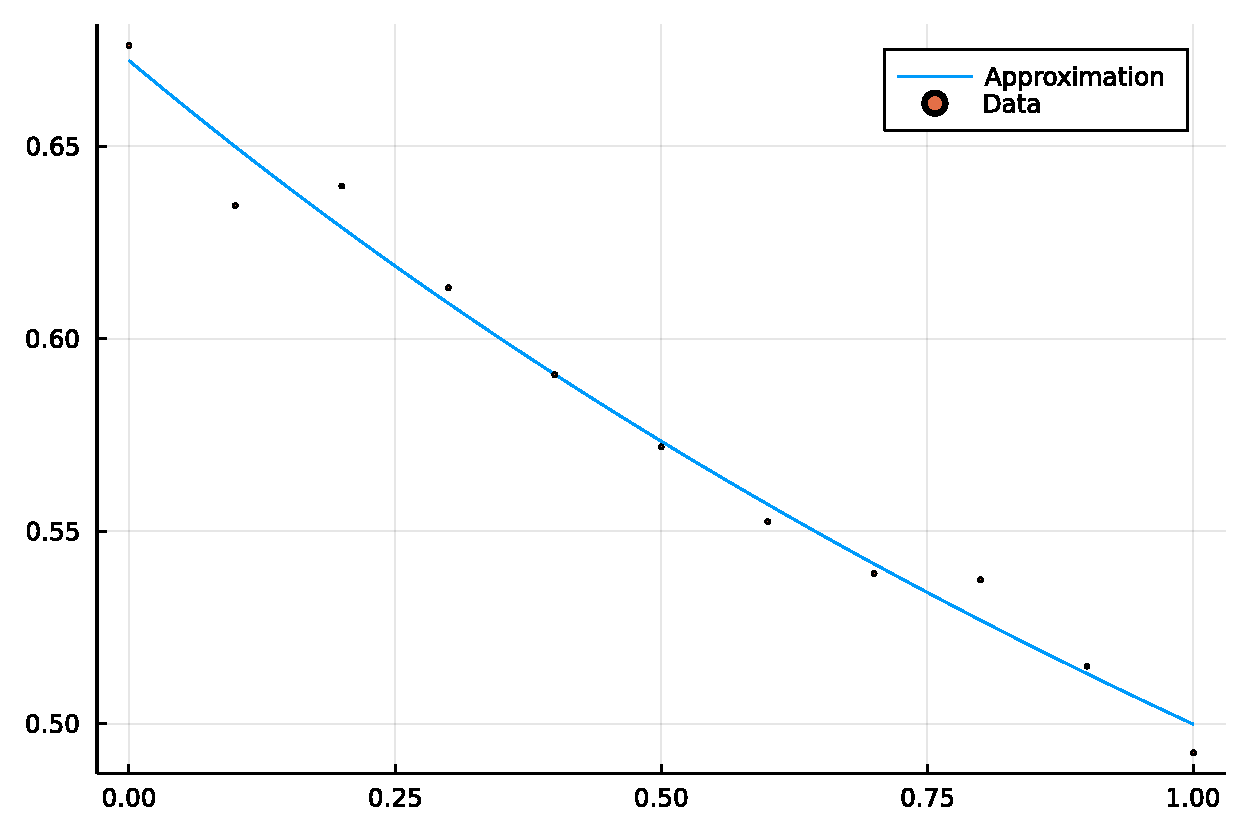
\includegraphics[width=0.6\linewidth]{figures/approx.pdf}
        \caption{Solution to \cref{exercise:nonlinear_approximation}.}%
        \label{fig:solution_exercise_approximation}
    \end{figure}
\end{exercise}

\begin{exercise}
    [Nonlinear least-squares]
    \label{exercise:nonlinear_least_squares}
    Suppose that we are given $n$ data points $(x_i, y_i)$ of an unknown function~$y = f(x)$.
    We wish to approximate $f$ by a straight line
    \[
        \widetilde f(x) = ax + b
    \]
    by minimizing the sum of squared \emph{Euclidean distances} between the data points and the straight line~$\widetilde f$.
    Since the distance between a point $(x_i, y_i)$ and the straight line is given by
    \[
        \frac{\lvert y_i - a x_i - b \rvert}{\sqrt{1+a^2}},
    \]
    the objective function to minimize is given by
    \[
        J(a, b) := \sum_{i=1}^{n} \frac{ \left( y_i - a x_i - b \right)^2 }{1+a^2}.
    \]
    This is a smooth function of~$a$ and $b$,
    and so a necessary condition for a pair $(a_*, b_*) \in \real^2$ to be a minimizer is that
    \[
        \nabla J(a_*, b_*) = \vect 0,
    \]
    which is a nonlinear equation for the unknowns~$a_*$ and $b_*$.
    Solve this equation by using the Newton--Raphson method initialized at~$(1, 1)$,
    and then plot the data points together with the function~$\widetilde f$ over the interval~$[0, 1]$.
    Your plot should look like \cref{fig:solution_exercise_approximation_least_squares}.
    The data is given hereafter:
    \begin{minted}{julia}
x = [0.0; 0.1; 0.2; 0.3; 0.4; 0.5; 0.6; 0.7; 0.8; 0.9; 1.0]
y = [-0.9187980789440975; -0.6159791344678258; -0.25568734869121856;
     -0.14269370171581808; 0.3094396057228459; 0.6318327173549161;
     0.8370437988106428; 1.0970402798788812; 1.6057799131867696;
     1.869090784869698; 2.075369730726694]
    \end{minted}
    \begin{figure}[ht]
        \centering
        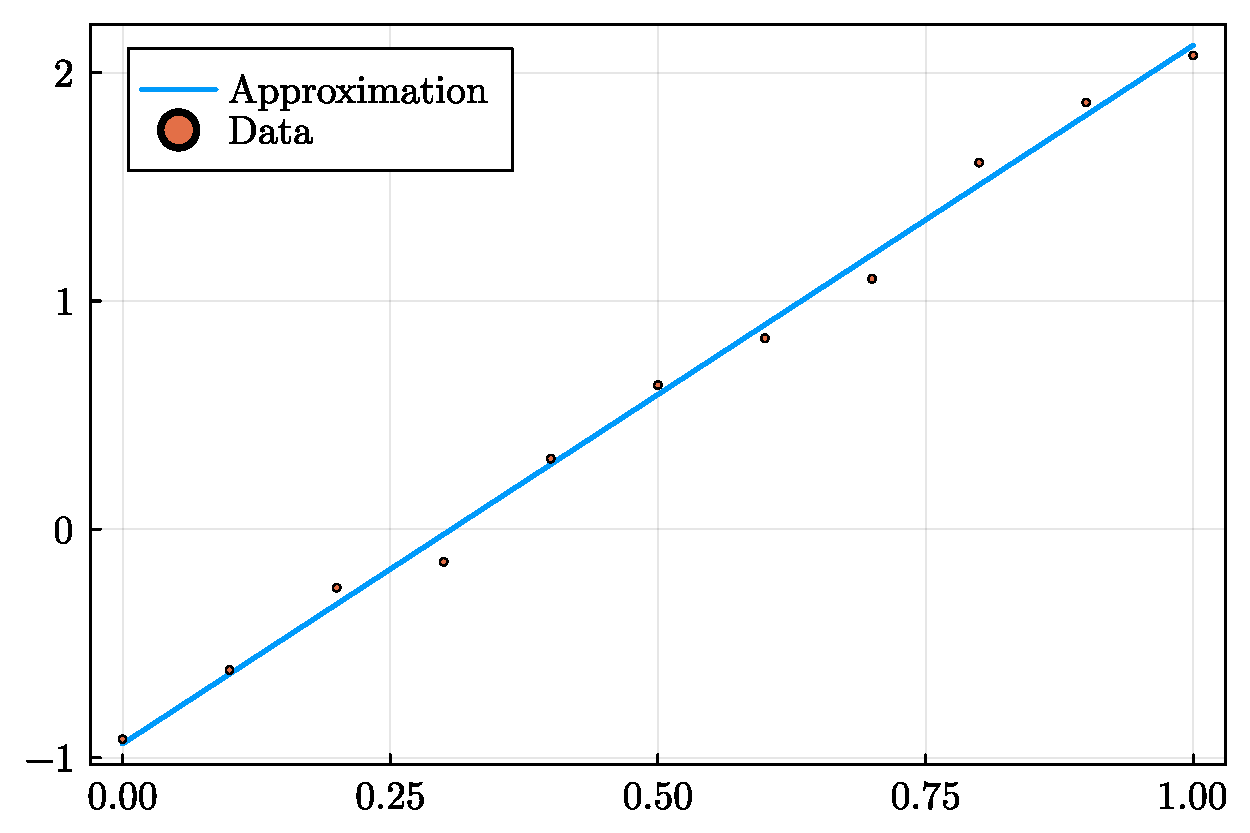
\includegraphics[width=0.6\linewidth]{figures/approx_line.pdf}
        \caption{Solution to \cref{exercise:nonlinear_least_squares}.}%
        \label{fig:solution_exercise_approximation_least_squares}
    \end{figure}
\end{exercise}

\section{Discussion and bibliography}

The content of this chapter is largely based on the lecture notes~\cite{VanDooren}.
Several of the exercises are taken or inspired from~\cite{Legat}.
The proof of convergence of the secant method is inspired from the general proof presented in the short paper~\cite{MR1186462}.
For a detailed treatment of iterative methods for nonlinear equations,
see the book~\cite{MR1744713}.
